\section{Julia Kempe and the collaboration environment}

\subsection{Positioning of the speaker}

As of June 2026, Julia Kempe's official academic page describes her as a researcher in the foundations of AI and machine learning, a Silver Professor at NYU's Courant Institute and Center for Data Science, currently on leave, and a Director and Senior Researcher at Meta FAIR, where she leads the Foundations of Reasoning Team (FoRT) \citep{kempebio2026,kempecv2026}. Her trajectory combines mathematics, theoretical computer science, quantum information, machine learning theory, data science leadership, and industrial research.

This matters for interpreting the lecture. The presentation is not a general advocacy talk about synthetic data. It is characteristic of a research environment that seeks mathematically tractable models, then validates them on controlled transformer and LLM experiments. The approach moves repeatedly between:

\begin{itemize}[leftmargin=*]
  \item asymptotic theory;
  \item simplified models that isolate one mechanism;
  \item algorithmic tasks with exact or interpretable structure;
  \item larger text-generation experiments;
  \item implications for data curation and future model training.
\end{itemize}

\subsection{Selected synthetic-data collaboration network}

The papers most directly connected to the lecture involve a recurring group of collaborators:

\begin{itemize}[leftmargin=*]
  \item Elvis Dohmatob;
  \item Yunzhen Feng;
  \item Pu Yang;
  \item Francois Charton;
  \item Arjun Subramonian;
  \item Julia Kempe.
\end{itemize}

The collaborations connect Meta FAIR, NYU's Center for Data Science and Courant Institute, and, in the verifier paper, Peking University \citep{dohmatob2024tails,dohmatob2024regression,feng2025verification,dohmatob2025strong}. The lecture itself belongs to the IHES/CNRS mathematics-and-LLM ecosystem \citep{ihesmathllm2024}.

\begin{figure}[H]
\centering
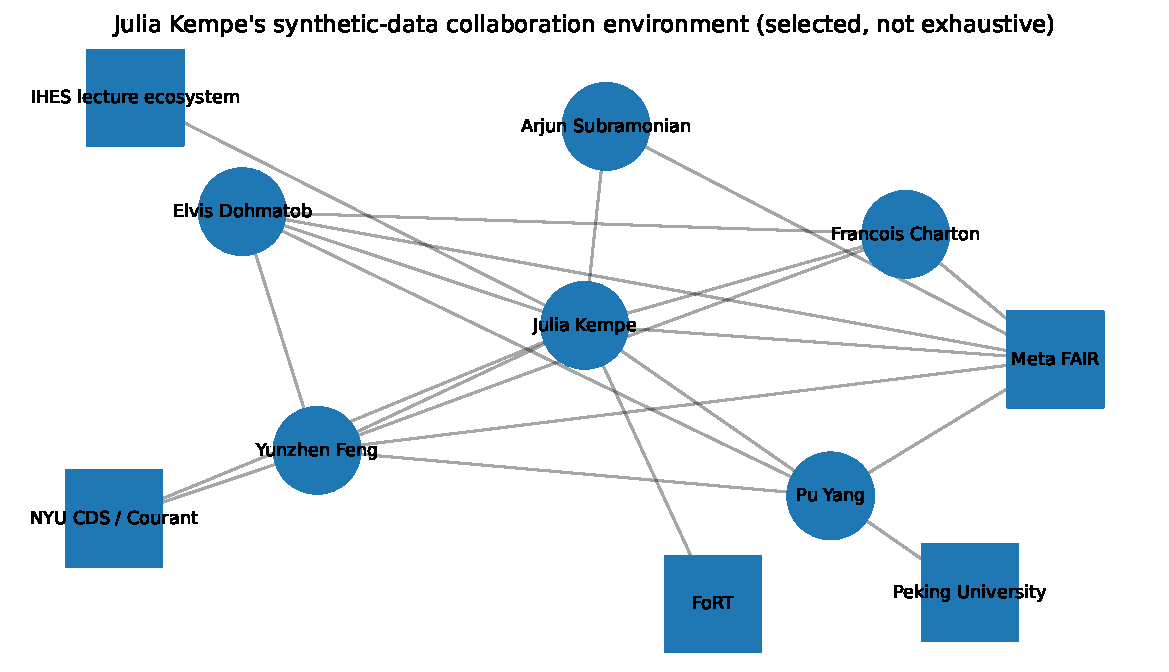
\includegraphics[width=0.96\textwidth]{figures/julia_collaboration_network.pdf}
\caption{Selected collaboration environment reconstructed from the cited synthetic-data papers and current institutional roles. It is intentionally not exhaustive.}
\label{fig:julia-network}
\end{figure}

\subsection{Why the team structure is scientifically relevant}

The research programme benefits from several complementary competencies.

\begin{longtable}{p{0.25\textwidth}p{0.30\textwidth}p{0.35\textwidth}}
\toprule
\textbf{Competence} & \textbf{Role in the programme} & \textbf{Visible contribution in the lecture line} \\
\midrule
Learning theory & Formalize generalization and asymptotics & Modified scaling laws and strong-collapse regimes \\
High-dimensional statistics & Separate bias, variance, spectrum and regularization & Kernel/ridge analysis \\
Interpretable mathematical tasks & Provide exact structure and controllable distributions & GCD and eigenvalue experiments \\
Large-model experimentation & Test whether toy-model mechanisms survive in LLM settings & Llama-based text-generation experiments \\
Verification theory & Characterize when filtering synthetic candidates helps & Verifier true/false acceptance analysis \\
Data-centric AI & Treat the corpus as a designed object rather than passive input & Tail preservation and collapse-aware curation \\
\bottomrule
\end{longtable}

The environment is therefore neither purely theoretical nor purely empirical. It resembles a loop:
\[
\text{mechanism hypothesis}
\rightarrow \text{tractable theorem}
\rightarrow \text{controlled experiment}
\rightarrow \text{larger-model test}
\rightarrow \text{new mechanism}.
\]

\subsection{A broader reasoning-and-mathematics context}

Kempe's current official role at Meta FAIR places the work in a broader Foundations of Reasoning environment. That environment is relevant to MMALS because it studies not only output quality but also the conditions under which reasoning, mathematical structure, verification, and data generation can scale. The synthetic-data papers should thus be read as part of a wider question:

\begin{quote}
How can a model generate, select, preserve, and improve structured knowledge without turning its previous approximations into an unquestioned source of truth?
\end{quote}

That question is directly aligned with MMALS memory consolidation, protocol verification, route selection, and functional specialization.

\subsection{Critical reading of authority}

The speaker's credentials and institutional environment justify taking the work seriously. They do not remove the need for critical evaluation. The models are deliberately simplified, practical pipelines vary, and later literature has shown that replacement, accumulation, verification, and mixture policies can lead to different outcomes.

The correct use of this research is therefore:

\begin{enumerate}[leftmargin=*]
  \item preserve the precise assumptions of each theorem;
  \item reproduce the controlled experiments;
  \item test whether the mechanism transfers to the target architecture;
  \item avoid using the prestige of the environment as a substitute for evidence.
\end{enumerate}
